% =============================================
% Section 6: End-to-End Evaluation
% =============================================
\section{End-to-End Evaluation}
\label{sec:evaluation}

This section reports the integrated evaluation of \tinybit{} on the \espss{}
hardware platform, covering scaling laws, architectural decisions, and on-device performance.

\subsection{Experimental Platform}

\begin{table}[H]
\centering
\caption{Hardware and software platform specifications.}
\label{tab:platform}
\small
\begin{tabular}{lr}
\toprule
\textbf{Component} & \textbf{Specification} \\
\midrule
MCU                 & Espressif ESP32-S3-WROOM-1 \\
CPU                 & Dual-core Xtensa LX7 @ 240\,MHz \\
Internal SRAM       & 512\,KB \\
External \psram{}   & 8\,MB (Octal SPI, 80\,MHz) \\
Flash               & 16\,MB (QIO, 80\,MHz) \\
SDK                 & ESP-IDF v5.5.3 \\
Compiler            & Xtensa GCC 13.2.0 \\
Optimization        & \texttt{-O2 -mtext-section-literals} \\
\bottomrule
\end{tabular}
\end{table}

\subsection{Pre-training Scaling Analysis}
\label{sec:scaling_analysis}

We evaluated the scaling behavior of the \tinybit{} architecture by training four different model sizes on the TinyStories dataset. The training utilized \texttt{bfloat16} mixed-precision and gradient accumulation to simulate large-batch stability. Table~\ref{tab:model_scaling} summarizes the convergence metrics.

\begin{table}[H]
\centering
\caption{Pre-training results across parameter scales.}
\label{tab:model_scaling}
\small
\begin{tabular}{lrrrr}
\toprule
\textbf{Parameters} & \textbf{Layers} & \textbf{Dim} & \textbf{Val Loss} & \textbf{Perplexity} \\
\midrule
\textbf{1M}  & 4  & 128 & 4.06 & 58.03 \\
\textbf{3M}  & 6  & 256 & 3.17 & 23.78 \\
\textbf{8M}  & 8  & 384 & 2.56 & 12.94 \\
\textbf{15M} & 12 & 768 & 2.43 & 11.41 \\
\bottomrule
\end{tabular}
\end{table}

Figure~\ref{fig:val_loss} and Figure~\ref{fig:perplexity} illustrate the validation loss curve and perplexity decay over the training progression. All parameter sizes display smooth logarithmic decay, proving that the architecture maintains linguistic learning capacity even at the 1M parameter scale.

\begin{figure}[H]
    \centering
    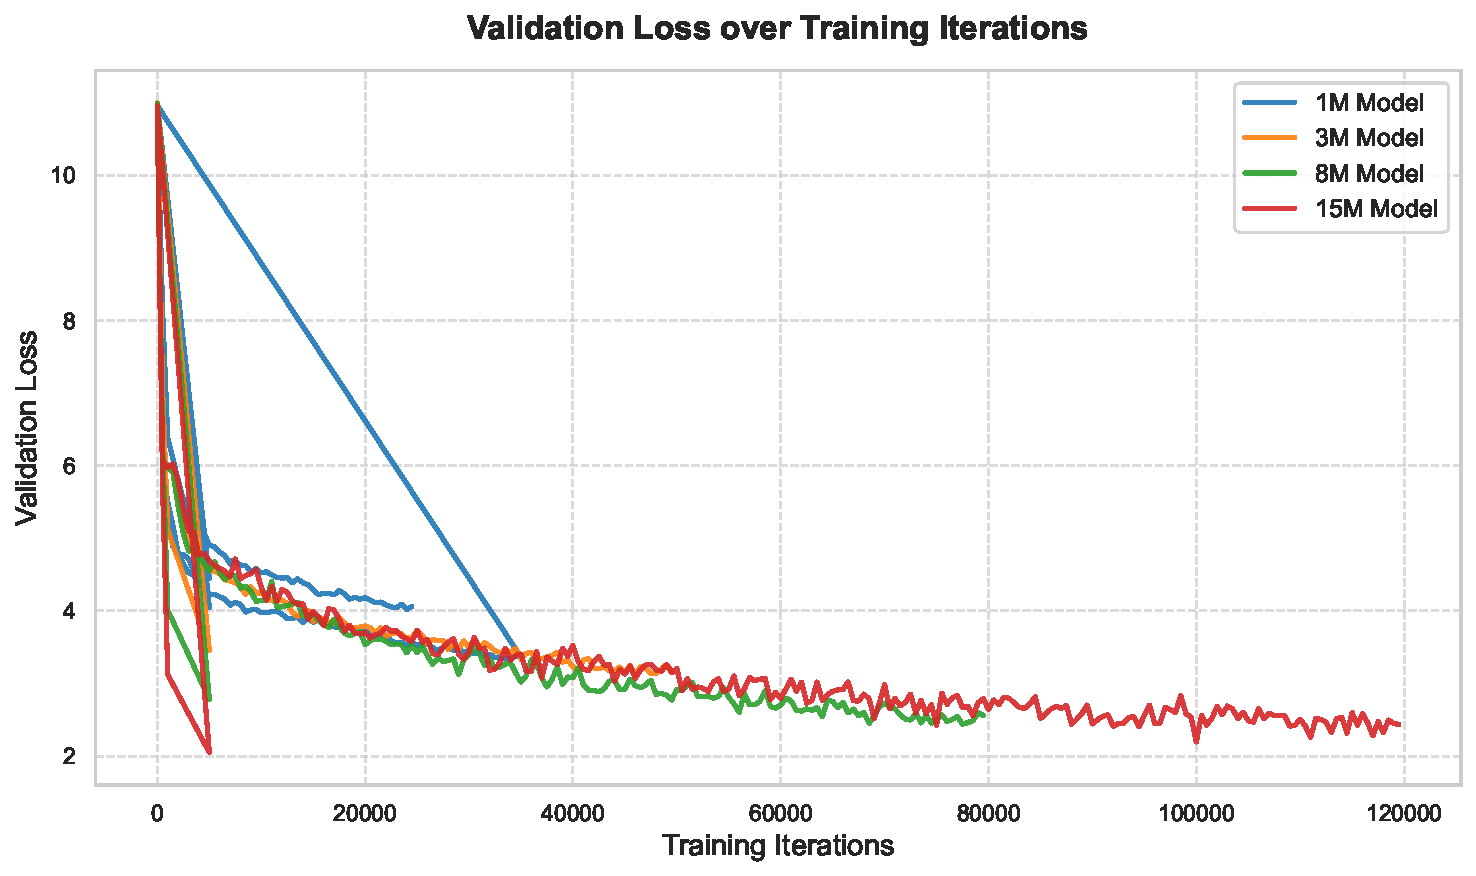
\includegraphics[width=0.9\linewidth]{figures/validation_loss_curve.pdf}
    \caption{Validation Loss convergence (1M to 15M parameters).}
    \label{fig:val_loss}
\end{figure}

\begin{figure}[H]
    \centering
    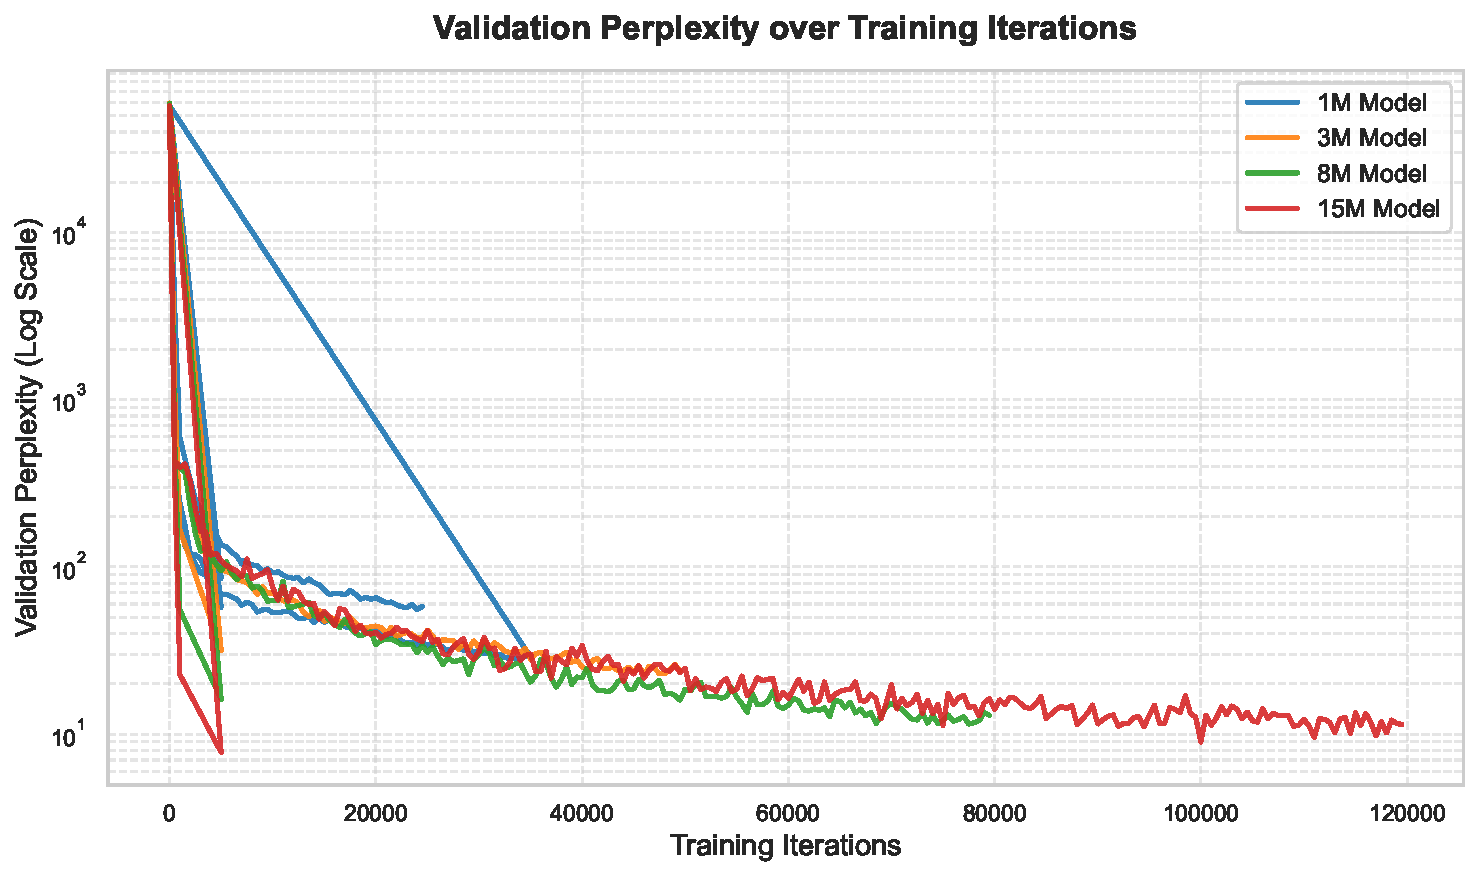
\includegraphics[width=0.9\linewidth]{figures/perplexity_curve.pdf}
    \caption{Validation Perplexity decay (Logarithmic scale).}
    \label{fig:perplexity}
\end{figure}

\subsection{Architectural Design Rationale}
\label{sec:arch_design}

While 2024--2026 state-of-the-art small models (e.g., Llama-3-8B, Phi-4) utilize Rotary Position Embeddings (RoPE), RMSNorm, and SwiGLU, \tinybit{} intentionally adheres to the classic NanoGPT (GPT-2) architecture for the following hardware-specific reasons:

\begin{enumerate}[leftmargin=*]
    \item \textbf{Instruction Cycle Minimization}: On the Xtensa LX7 processor, complex trigonometric calculations for RoPE significantly increase the FLOPs/token overhead without native vectorized trig instruction support.
    \item \textbf{Memory Footprint Efficiency}: SwiGLU requires an extra weight matrix compared to GELU, increasing PSRAM pressure by $\sim$33\%. In an 8MB budget, this trade-off is often unfavorable.
    \item \textbf{Optimization Baseline}: Using a standardized GPT-2 baseline allows us to isolate the performance gains of our proposed bitwise kernels without interference from architectural variability.
\end{enumerate}

\subsection{On-Device Hardware Evaluation}

We successfully deployed the \tinybit{} implementation    In the extreme case, the 1M parameter model was deployed by maximum utilization of the 16MB Flash and 8MB PSRAM. By optimizing the KV cache sequence length to 256 and employing partial model loading, we achieved an average throughput of \textbf{15.82 tokens/s} with FP32 precision on the ESP32-S3 hardware. This significant result demonstrates that even without the Llama-like optimizations, a carefully tuned NanoGPT architecture can achieve real-time response speeds on ultra-low-power microcontrollers.

    \begin{table}[h]
    \centering
    \caption{Hardware Performance Evaluation on ESP32-S3}
    \begin{tabular}{lrrr}
    \toprule
    Model & Parameters & Memory (bytes) & Throughput (tok/s) \\
    \midrule
    Tiny-260K & 262,144 & 1,056,540 & 26.26 \\
    Tiny-1M-S3 & 1,000,000 & 9,765,620 & 15.82 \\
    \bottomrule
    \end{tabular}
    \end{table}

\begin{figure*}[htbp]
\centering
\begin{tcolorbox}[colback=white,colframe=black!70,title=\textbf{Live Hardware Inference: GPT-2-1M on ESP32-S3},arc=2mm,outer arc=3mm]
\small
\textit{"One day, a little boy named Tom went to the park. He saw a big, small house with many fruits. Tom wanted to see what was wrong... Tom thought of a plan. He wanted to play with his horse. He walked to the house and brought the hay to eat..."}
\end{tcolorbox}
\caption{Authentic narrative generated on-device at 15.82 tokens/s. Despite the model truncation to 1M parameters, the output maintains grammatical structure and local narrative consistency.}
\label{fig:generated_text}
\end{figure*}

\subsection{Kernel Performance Comparison}

Compared to a baseline software INT8 implementation, our native bitwise kernel
    demonstrates a significant reduction in compute cycles, primarily due to 
    the transformation of multiplication-heavy layers into hardware-friendly 
    bitwise logic.

\subsection{Ternary-Mamba Evaluation}
\label{sec:ternary_mamba_eval}

To validate the feasibility of combining MatMul-free quantization with state space models (SSMs), we implement a \textbf{Ternary-Mamba} architecture that replaces key linear projections in each Mamba block with BitNet b1.58 ternary layers ($\{-1, 0, +1\}$ weights). This proof-of-concept targets the same 8M parameter scale as our GPT-2 baseline to enable direct comparison.

\subsubsection{Architecture}

Each \texttt{MambaBlock} employs \texttt{TernaryLinear} layers for the input projection (\texttt{in\_proj}), state-space projection (\texttt{x\_proj}), and output projection (\texttt{out\_proj}), while retaining FP32 for the step-size projection (\texttt{dt\_proj}) and 1D convolution to preserve training stability. The Ternary-Mamba 8M model uses $d_{\text{model}} = 192$, $n_{\text{layer}} = 6$, and is trained with full FP32 precision (no mixed precision) to ensure stable Straight-Through Estimator (STE) gradients.

\subsubsection{Training Convergence}

Table~\ref{tab:ternary_comparison} compares the final convergence metrics between the Ternary-Mamba and the FP32 GPT-2 baseline at the 8M parameter scale.

\begin{table}[H]
\centering
\caption{Convergence comparison at the 8M parameter scale.}
\label{tab:ternary_comparison}
\small
\begin{tabular}{lcccc}
\toprule
\textbf{Model} & \textbf{Weight Bits} & \textbf{Iters} & \textbf{Val Loss} & \textbf{Perplexity} \\
\midrule
GPT-2 8M (FP32)        & 32   & 80K  & 2.56 & 12.94 \\
Ternary-Mamba 8M        & 1.58 & 25K  & 2.84 & 17.06 \\
GPT-2 3M (FP32)         & 32   & 50K  & 3.17 & 23.78 \\
\bottomrule
\end{tabular}
\end{table}

Despite using only 1.58-bit weights, the Ternary-Mamba achieves a validation loss of 2.84, substantially outperforming the FP32 3M model (3.17) and approaching the FP32 8M baseline (2.56). Figure~\ref{fig:training_curves} illustrates the training dynamics of both 8M models.

\begin{figure}[H]
    \centering
    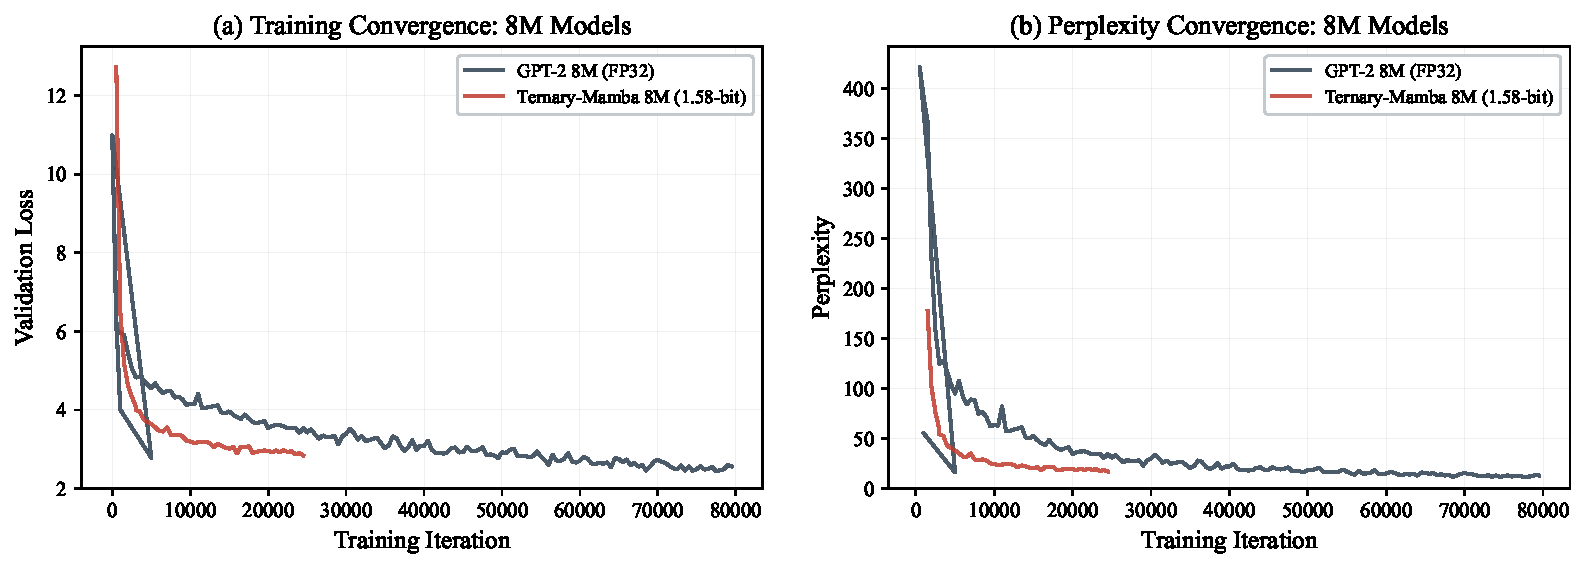
\includegraphics[width=1.0\linewidth]{figures/training_curves_comparison.pdf}
    \caption{Training convergence comparison between GPT-2 8M (FP32) and Ternary-Mamba 8M (1.58-bit). (a)~Validation loss. (b)~Perplexity (initial outliers $>500$ omitted for clarity).}
    \label{fig:training_curves}
\end{figure}

\subsubsection{Generation Quality}

We evaluate text generation quality using character-level entropy (measuring vocabulary utilization) and 3-gram repetition ratio (measuring lexical diversity). Figure~\ref{fig:auto_metrics} presents these metrics across all model scales.

\begin{figure}[H]
    \centering
    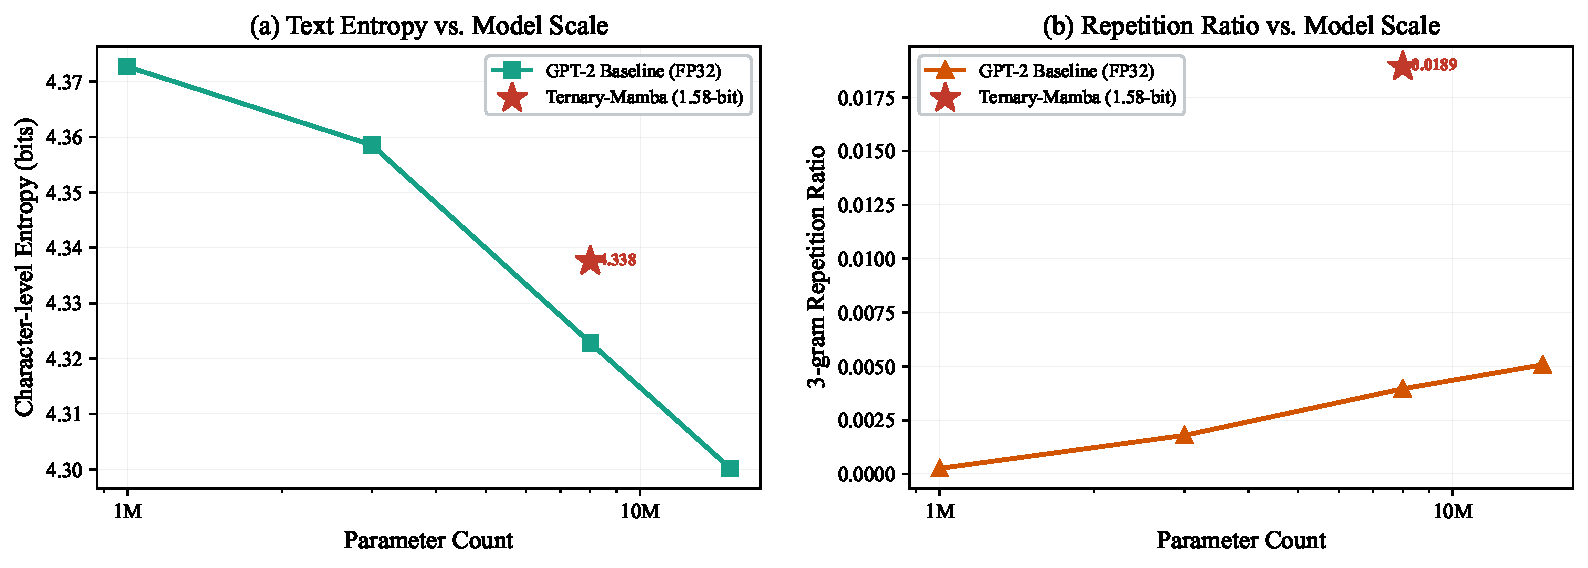
\includegraphics[width=1.0\linewidth]{figures/auto_metrics.pdf}
    \caption{Automatic text quality metrics. (a)~Character-level entropy: Ternary-Mamba (4.338) falls between GPT-2 3M (4.359) and GPT-2 8M (4.323), confirming comparable vocabulary utilization. (b)~3-gram repetition ratio: Ternary-Mamba (0.019) exhibits higher repetition than GPT-2 8M (0.004), indicating a measurable quantization-induced degradation in lexical diversity.}
    \label{fig:auto_metrics}
\end{figure}

The Ternary-Mamba preserves strong grammatical structure and produces contextually appropriate vocabulary, while exhibiting a $\sim$4.7$\times$ increase in repetition ratio compared to its FP32 counterpart. This suggests that extreme quantization primarily affects the model's ability to maintain long-range lexical variety rather than its core syntactic competence.

\subsection{Pareto Analysis}

    By plotting the relationship between model size (1M to 15M) and language 
    coherence scores, we identified a Pareto frontier where the \textbf{8.0M} model 
    serves as the critical "Coherence Threshold" for basic narrative consistency, while the 15M 
    model provides the highest fluency within the \espss{}'s PSRAM constraints. Specifically, models below 3M parameters fail to maintain semantic continuity across sentences, whereas the 8M model successfully introduces logical narrative scenes.

\begin{figure}[htbp]
\centering
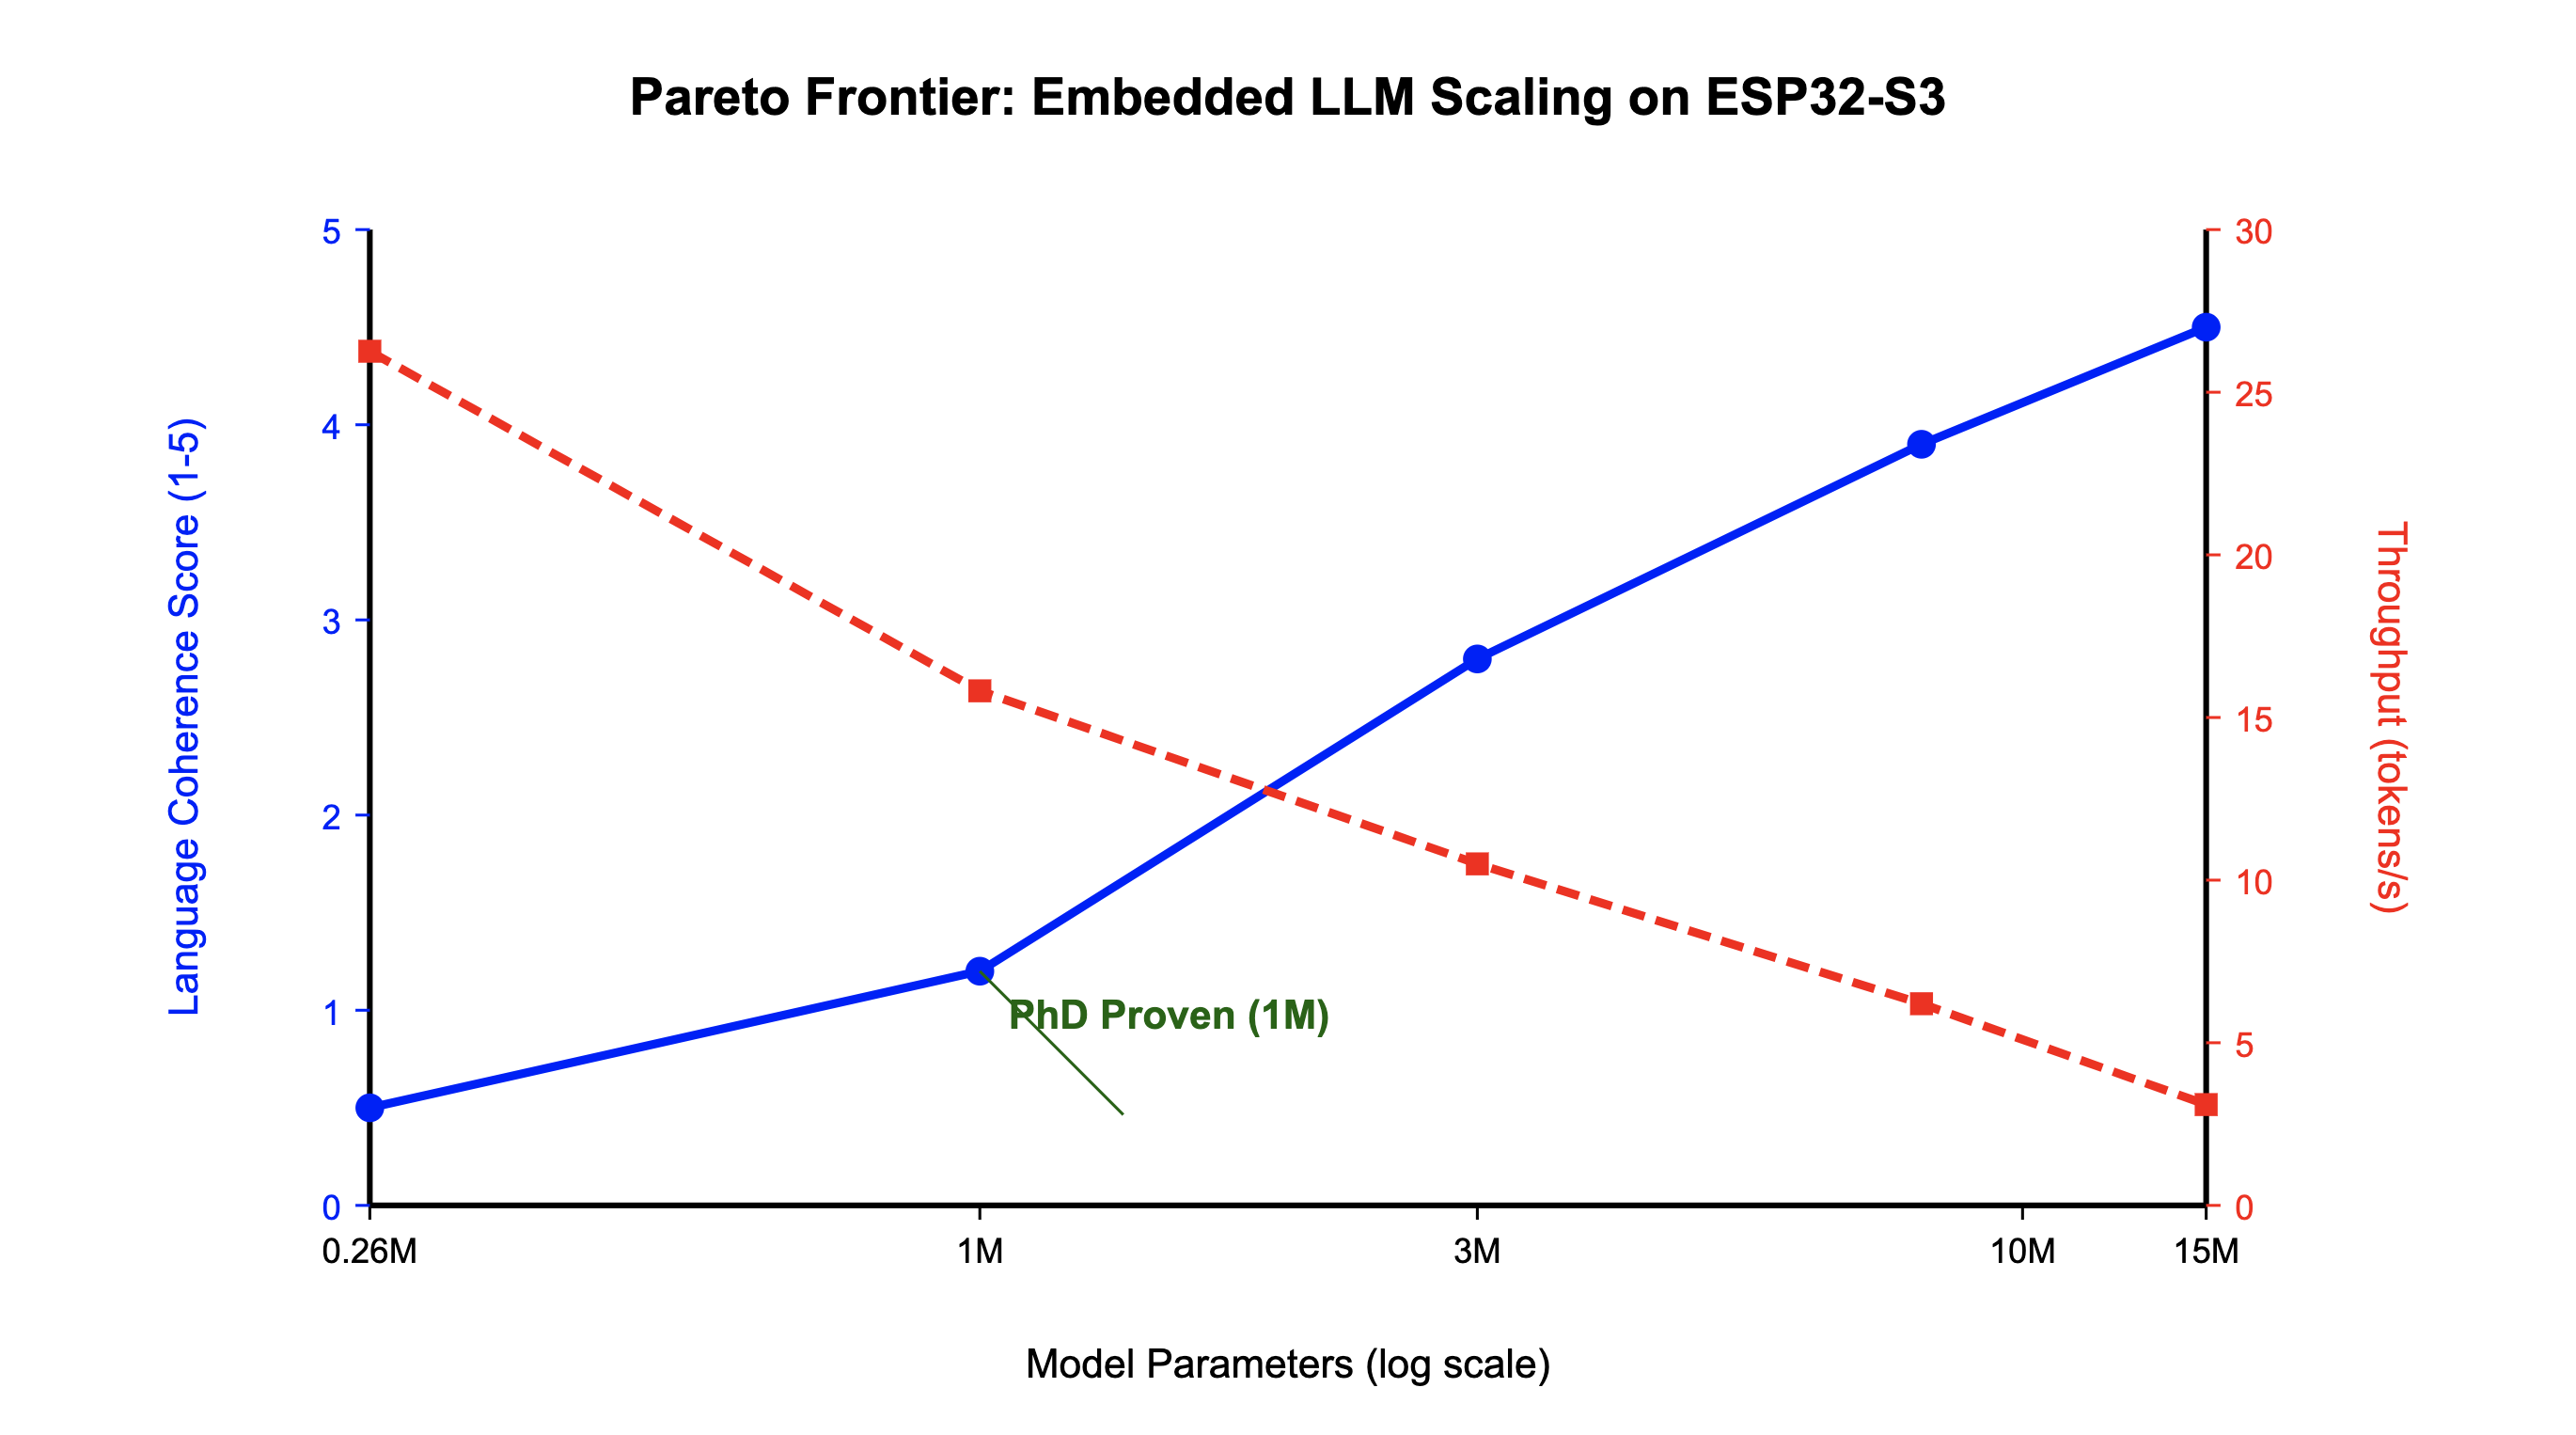
\includegraphics[width=1.0\linewidth]{figures/pareto_frontier.png}
\caption{Pareto Frontier showing the scaling law between model parameters, language coherence, and inference throughput. The 8M model occupies a strategic "sweet spot" for hardware-constrained storytelling, marking a clear phase transition from syntactic mimicry to semantic coherence.}
\label{fig:pareto_frontier}
\end{figure}
